\documentclass[english,hidelinks,pdftex, 11 pt, class=report,crop=false]{standalone}
\usepackage[T1]{fontenc}
\usepackage[utf8]{luainputenc}
\usepackage{lmodern} % load a font with all the characters
\usepackage{geometry}
\geometry{verbose,a4paper, inner=0cm, outer=0 cm, bmargin=2cm, tmargin=1cm}
%\textwidth=12cm
\setlength{\parindent}{0bp}
\usepackage{import}
\usepackage[subpreambles=false]{standalone}
\usepackage{amsmath}
\usepackage{amssymb}
\usepackage{esint}
\usepackage{babel}
\usepackage{tabu}
\usepackage[dvipsnames, table]{xcolor}
\usepackage{cancel}
\makeatother
\makeatletter
\usepackage{datetime2}
\usepackage{titlesec}
\usepackage[many]{tcolorbox}

% Eheter
\newcommand{\enh}[1]{\,\textrm{#1}}
%referances
\newcommand{\net}[2]{{\color{blue}\href{#1}{#2}}}

%Spaces
\newcommand{\vsk}{\\[12pt]}
\newcommand{\vs}{\vspace{-12pt}}

% Tabell for opplegg

\newcommand{\ovlist}[1]{
\vspace{-16pt}
\begin{itemize}
	#1
\end{itemize}
}

% Chapters and sections
\titleformat{\section}[block]{\bfseries}{\hspace{3cm}\thesection}{5pt}{}
\titleformat{\subsection}[block]{\bfseries}{\hspace{3cm}\thesection}{5pt}{}
\newcommand{\sectionbreak}{\clearpage} % New page on each section
 

\newlength{\mywidth}
\setlength{\mywidth}{14cm}

\newcommand{\cont}[1]{
\begin{tcolorbox}[center, boxrule=0.0 mm, width=\mywidth,arc=0mm,enhanced jigsaw,,colback=white,breakable]
#1	
\end{tcolorbox}
}

\newcommand{\info}[5]{
\begin{tcolorbox}[center, boxrule=0.1 mm, width=\mywidth,arc=0mm,enhanced jigsaw,breakable,colback=yellow!5]	
	
	\footnotesize
	\textbf{Øvingsområde}\\[5pt] #1 
	
	\textbf{Utstyr}\\ #2  \\
	
	\begin{tabular}{@{} p{4cm} p{4cm} l} 
		\textbf{Tid} & \textbf{Elevinndeling} & \textbf{Læringsarena} \\
		#3  & #4 & #5
	\end{tabular} 
\end{tcolorbox}	
}

\newcommand{\gjen}[1]{\begin{tcolorbox}[center,boxrule=0.1 mm, width=\mywidth,arc=0mm,colback=blue!3] {\large \textbf{Gjennomføring} \vspace{5 pt}}\newline #1  \end{tcolorbox}\vspace{-5pt}}
\newcommand{\eks}[1]{\begin{tcolorbox}[center,boxrule=0.1 mm, width=\mywidth,arc=0mm,colback=green!3] {\large \textbf{Eksempel} \vspace{5 pt}}\newline #1  \end{tcolorbox}\vspace{-5pt}}

\newcounter{opl}
%\numberwithin{opl}{article}


\newcommand{\opl}[1]{
\newpage
{\refstepcounter{opl} %\phantomsection 
\large \textbf{\theopl \;#1} \vsk}
}

% Headlines
\newcommand{\fork}{\textbf{Forkunnskapar}\\}
\newcommand{\forb}{\textbf{Forberedelsar}\\}
\newcommand{\opgvr}{\textbf{Oppgaver}}



%colors
\newcommand{\colr}[1]{{\color{red} #1}}
\newcommand{\colb}[1]{{\color{blue} #1}}
\newcommand{\colo}[1]{{\color{orange} #1}}
\newcommand{\colc}[1]{{\color{cyan} #1}}
\definecolor{projectgreen}{cmyk}{100,0,100,0}
\newcommand{\colg}[1]{{\color{projectgreen} #1}}

% Lister med bokstavar
\usepackage[inline]{enumitem}
% Opg
\newcommand{\abc}[1]{
	\begin{enumerate}[label=\alph*),leftmargin=18pt]
		#1
	\end{enumerate}
}

\usepackage[]{hyperref}

\begin{document}

\section{Følger og rekker}
\subimport{/home/sindre/precalc/ggb/}{ncmd}
\rgg{{\large \texttt{Regresjonsanalyse} (Regneark) \gvs\\}
Analyse av tallfølge skrevet inn i regnearket for å finne en eksplisitt formel.
}
\eks{
Finn den eksplisitte formelen til følgen
\[ 2,6, 22, 56, 114, 202, ...  \]
\sv
Vi velger
{\tt Vis $ \blacktriangleright $ Regneark} og skriver tallene inn i en tabell med leddnummeret i første kolonne og verdien i andre.
\begin{figure}[H]
	\centering
	\includegraphics[scale=0.5]{fig/regf}
\end{figure}
Vi markerer så hele tabellen, i verktøymenyen som da dukker opp, velger vi {\tt Regresjonsanalyse}. 
\begin{figure}[H]
	\centering
	\includegraphics[scale=0.5]{fig/regf2}
\end{figure}
På vinduet som da kommer velger vi {\tt Analyser}, og trykker deretter på {\tt Vis statistikk} \big(\,\includegraphics[scale=0.4]{fig/stat0}\,\big). I analysevinduet søker vi nå å finne en {\tt Regresjonsmodell} hvor vi får\footnote{$\, \tt R^2 $ er et mål på hvor godt modellen samsvarer med inputen, gitt som en skala mellom 0 og 1. 1 betyr fullstendig samsvar.} $ \tt {R^2 = 1}$  i statistikkvinduet. I dette tilfellet gir et tredjegradspolynom det vi ønsker:
\begin{figure}[H]
	\centering
	\includegraphics[scale=0.6]{fig/stat}
\end{figure}
Av $ {y =x^3 - 3x+4} $ i figuren over konkluderer vi med at den eksplisitte formelen til følgen er:
\[ a_n = n^3 -3n +4 \] \vs\vs
}

\rgg{\summ}
\eks{
	Finn summen av den uendelige rekka
	\[ 1+ \frac{1}{5} + \frac{1}{25} +...  \]	
	
	\sv
	Dette er en geometrisk rekke med $ {k=\frac{1}{5}} $ og eksplisitt formel gitt som:
	\[ a_n = \frac{1}{5^{(n-1)}} \] 	
	for $ {n\in\mathbb{N}} $. \vsk
	
	I CAS skriver vi da ($ \infty $-tegnet finner du ved å trykke på $ \alpha$-tegnet oppe i høyre hjørne):
	\begin{center}
		\includegraphics[scale=0.5]{fig/rek}
	\end{center}
	
}

\section{Trigonometri}
\rgg{\los}
\eks[1]{
	\vs
	\begin{figure}
		\centering
		\includegraphics[scale=0.5]{fig/trilig}
	\end{figure}	
	I \textit{Før Kalkulus; Teoridel}  brukes $ {n\in \mathbb{Z}} $ som heltallsvariabel, GeoGebra bruker en indeksert $ k $ (her $ {k_1 \in \mathbb{Z}})$.
	
	\merk Du kan også løse ligningen ved å skrive den inn i en celle og deretter trykke på \texttt{Løs}.
}
\eks[2]{
Løs ligningen 
\[ \cos^2(3x)-3 \cos(3x)-4 =0 \]
\sv \vs
\fig{trilig2}
\textsl{Merk}: Løsningen kan komprimeres til (forklar for deg selv hvorfor):
\[ x=\frac{1}{3}\pi(2k+1)\]
for $ k\in \mathbb{Z} $.
}
\newpage
\rtrikomb
\eks{
		\centering
		\includegraphics[scale=0.5]{\scr{trikomb}}

}
\rregsin
\eks{
	Gitt tabellen \vs
	\begin{center}
		\begin{tabular}{|c | c|}
					\hline
				$ x $ & $ f(x) $ \\		
			\hline			
			0 & 0 \\
			\hline
			1 & -2.12 \\
			\hline
			2 & -2.73 \\
			\hline
			3 & -0.62 \\
			\hline
			4 & 2.37 \\
			\hline
			5 & 2.88\\	
			\hline	
		\end{tabular}
	\end{center}
	Bruk regresjon for å finne en tilnærming til $ f(x) $ uttrykt som en sinusfunksjon. \vsk
	
	\sv	
	Vi velger
	{\tt Vis $ \blacktriangleright $ Regneark} og skriver inn tabellen. Vi markerer så begge kolonner, høyreklikker innenfor markeringsfeltet og velger \\{\tt Lag $ \blacktriangleright $ Liste med punkt}:
	\begin{figure}
		\centering
		\includegraphics[scale=0.5]{fig/reg}
	\end{figure} 
	Om vi ønsker at alle punktene skal vises i grafikkfeltet, høyreklikker vi på grafikken og velger {\tt Vis alle objekt}. Deretter skriver vi {\tt RegSin[Liste1]} i kommandolinjen, og får funksjonen {\tt f(x)} i algebrafeltet og grafen til \texttt{f} i grafikkfeltet. Denne funksjonen er en tilnærming til $ f(x) $ gitt i oppgaven.
	\begin{figure}
		\centering
		\includegraphics[scale=0.5]{fig/reg2}
	\end{figure} 
}
\section{Vektorer i rommet}
\rgg{\punkt \vs}
\rgg{\vektor}
\eks{
	Gitt vektorene $ {\vec{u}=[-4, 2, 7]} $, ${\vec{v}=[4, 6+s, -(s+t)]} $ og $ \vec{w}=[12, 2t-9s,\\ 3s-t]  $.\vsk
	
	\textbf{a)} Finn $ s $ og $ t $ slik at $ \vec{v}||\vec{w} $.\\
	\textbf{b)} Bestem $ s $ slik at ${ \vec{u}\perp\vec{v}} $ når $ {t=-2} $. \vsk
	
	\sv
	\textbf{a)}
	Det er en litt spesiell sak i CAS at en vektor $ [x, y, z] $ definert ved å skrive \texttt{(x, y, z)} vil ha en bedre funksjonalitet enn hvis den defineres ved \texttt{Vektor}-kommandoen. Vi starter derfor med å definere $ \vec{v} $ og $ \vec{w} $ på følgende måte (se \hr{Definere variabler}{defvar}):
	\begin{figure}[H]
		\centering
		\includegraphics[scale=0.5]{fig/vogw}
	\end{figure}
	Vi utnytter videre at $ {\vec{v}||\vec{w}}$ hvis $ {r\vec{v}=\vec{w}} $, for en konstant $ r $. Vi skriver denne ligningen inn i CAS og trykker så på \texttt{Løs}:
	\begin{figure}[H]
		\centering
		\includegraphics[scale=0.5]{fig/rv}
	\end{figure}
	Vi har altså at $ {s=-1} $ og $ {t=3} $. \vsk
	
	\textbf{b)} Skal $ {\vec{u }\perp \vec{v}}$, må vi ha at $ {\vec{u}\cdot\vec{v}=0} $. Vi definerer $ \vec{u} $ og bruker \texttt{ByttUt}-kommandoen for å sette $ {t=2} $ i uttrykket til $ \vec{v} $. Med det endrede uttrykket løser vi ligningen for skalarprduktet (se kommandoen \texttt{Skalarprodukt} på s. \pageref{skalgeo}. CAS fjerner \texttt{*} når vi skriver \texttt{u*\$5}). 
	\begin{figure}[H]
		\centering
		\includegraphics[scale=0.5]{fig/uskalvgeo}
	\end{figure}
}
\rskalar
\rvekpro
%\rdeter
%\rdetere
\rgg{\vink}
%\eks{
%\centering
%\includegraphics[scale=0.6]{\scr{vink}}
%}
\section{Romgeometrier}
\rpyr
\rh
\eks{
	Finn volumet og høyden til tetraetedet med grunnflate gitt ved punktene $ {A=(3, 2, 1)} $, $ {B=(6, 2, 1)} $, $ {C=(3, 6, 1)} $ og toppunkt ${ D=(5, 4, 3)} $.\vsk
	
	\sv
	Vi skriver inn punktene og bruker deretter kommandoen \texttt{Pyramide[A, B, C, D]} for å lage tetraedet $ a $. Algebrafeltet gir oss da at volumet til $ a $ er 4. I celle 1 finner vi høyden, som er 2.
	\begin{figure}
		\centering
		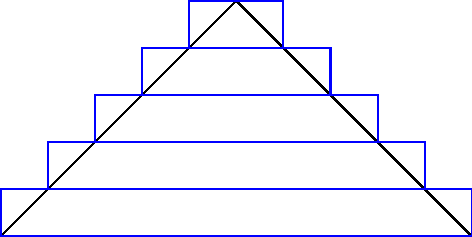
\includegraphics[scale=0.5]{fig/pyr}
	\end{figure}	
}
\rpris
\rkurve
\rlinje
\eks{Finn parameteriseringen til linjen som går mellom punktet $ {(-2, 1, 3)}$ og ${ (-5, -1, 4)} $. \vsk
	
	\sv
	Vi skriver punktene i inntastingsfeltet og får punktene $ A $ og $ B $. Etterpå skriver vi \texttt{Linje[A, B]} og får da linjen $ f $.
	\begin{figure}
		\centering
		\includegraphics[scale=0.5]{fig/linje}
	\end{figure}
	Av dette finner vi at parameteriseringen til linjen er gitt som:
	\[f: \left\lbrace{
		\begin{array}{lll}
		x=-2 -3t   \\
		y= 1 -2t    \\
		z= 3 + t 
		\end{array}
	}\right. \]	
}
\rkuler
\eks{
	En linje $ l $ med parameteriseringen
	\[l: \left\lbrace{
		\begin{array}{lll}
		x=-3 -2t   \\
		y= 1 +t    \\
		z= 4 + 2t 
		\end{array}
	}\right. \]	
	skjærer en kule med med sentrum i $ {(-1, 2, 6) }$ og radius lik 3. \vsk
	
	\textbf{a)} Tegn kulen og linjen.
	
	\textbf{b)} Finn skjæringspunktet mellom kulen og linjen. \vsk
	
	\sv
	Vi skal her se på to løsningsmetoder. Den første metoden er helt klart den raskeste, men den andre metoden er tatt med for å illustrere bruken av \texttt{Kurve}-kommandoen, i tillegg til å presentere en metode som vil sikre oss eksaktverdier.\vsk
	
	\textit{Løsningsmetode 1}\vsk
	
	\textbf{a)} 
	\begin{figure}
		\centering
		\includegraphics[scale=0.5]{fig/skjlinkul}
	\end{figure}
	Vi starter med å tegne kulen. I inntastingsfeltet skriver vi \texttt{Kule[(-1, 2, 6), 3]} og får kulen $ a $ i algebrafelt og grafikkfelt 3D. For å tegne linjen, skriver vi
	\texttt{(-3, 1, 4)+t*(2,1,2)} i inntastingsfeltet, resultatet er kurven $ f $.\vsk
	
	\textbf{b)}
	\begin{figure}
		\centering
		\includegraphics[scale=0.5]{fig/skjlinkulb}
	\end{figure}
	I inntastingsfeltet skriver vi \texttt{Skjæring[a, f]} og får de to punktene $ A $ og $ B $. 
	
	\merk Hadde vi tegnet linjen ved hjelp av \texttt{Kurve}-kommandoen, ville ikke dette funket. \texttt{Skjæring} er ikke kompatibel med \texttt{Kurve}, og i dette tilfellet heller ikke med CAS.\vsk
	
	\textit{Løsningsmetode 2}\vsk
	
	\textbf{a)} 
	\begin{figure}
		\centering
		\includegraphics[scale=0.5]{fig/skjlinkul2}
	\end{figure}
	For å tegne linjen, skriver vi \texttt{Kurve[-3 + 2t, 1 + t, 4 + 2t, t, -10, 10]} i inntastingsfeltet. At ${ t\in[-10, 10] }$ velger vi ut ifra inspeksjon i grafikkfelt 3D. Det gjelder å velge et intervall som viser begge skjæringspunktene mellom kulen og linjen (man kan velge $ {t\in[-\infty, \infty] }$, men da blir ikke kurven vist grafikkfeltet). Resultatet er kurven $ b $.\vsk
	
	\textbf{b)} (Se \hr{Høyre- og venstresiden}{hogl})\vs
	\begin{figure}
		\centering
		\includegraphics[scale=0.5]{\scr{skjlinkulb2}}
	\end{figure}
	I celle 1 lager vi oss en ny funksjon $ {k(x, y, z) }$ med et uttrykk tilsvarende venstresiden til kuleligningen. For at linjen skal skjære kulen, må parameteriseringen til linjen oppfylle kuleligningen. I celle 2 setter vi derfor uttrykkene for $ x, y $ og $ z $ fra parameteriseringen inn i $ k $, og krever at dette uttrykket skal bli lik $ 3^2 $. Vi trykker så på \texttt{Løs}-knappen og får to svar for $ t $. I celle 3 og 4 finner vi punktene for dissse valgene av $ t $.		
}
\rplan
\section{Derivasjon og funksjonsdrøfting}
\deru
\eks{\vs
\centering
\includegraphics[scale=0.5]{fig/fder}
}
\rvend
\eks{\vs
	\centering
	\includegraphics[scale=0.5]{fig/vend}
}
\rgg{\absmaks}
\rgg{\absmin}
\rgg{\ekstpkt}
\section{Integrasjon}
\rintu
\eks{
	\vs\vs
	\begin{figure}
		\centering
		\includegraphics[scale=0.5]{\scr{int}}
	\end{figure}	\vs
	$ c_1 $ er en vilkårlig konstant.
}
\rintb
\eks[1]{
	\vs \vs
	\begin{figure}
		\centering
		\includegraphics[scale=0.5]{\scr{intb}}
	\end{figure}	\vs
}
\eks[2]{
	Finn volumet av omdreiningslegemet til $ {f(x)=x^2 }$ på intervallet $ {[0, 1]} $. \vsk
	
	\sv \vs
	\begin{figure}
		\centering
		\includegraphics[scale=0.5]{\scr{omdr}}
	\end{figure}	
	I celle 1 definerer vi $ f(x) $. Volumet er gitt som ${\pi \int\limits_0^1 (f(x))^2\,dx} $, som vi finner i celle 2.		
}

\section{Differensialligninger}
\rdif
\eks[1]{
	Løs ligningen:
	\[ y'+2y=2 \]
	\sv \vs
	\begin{figure}
		\centering
		\includegraphics[scale=0.5]{\scr{dif1}}
	\end{figure}	
	$ c_1 $ er en vilkårlig konstant.
}
\eks[2]{
	Løs ligningen:
	\[ y'+5y^2=0 \]
	\sv \vs 
	\begin{figure}
		\centering
		\includegraphics[scale=0.5]{\scr{dif2}}
	\end{figure}	
	$ c_1 $ er en vilkårlig konstant.
}
\eks[3]{
	Løs ligningen:
	\[ y''+y'-6y=0 \]
	\sv \vs 
	\begin{figure}
		\centering
		\includegraphics[scale=0.5]{\scr{dif4}}
	\end{figure}	
	$ c_1 $ og $ c_2 $ er vilkårlige konstanter.
}
\rdiff
\eks[1]{
	Finn løsningen av ligningen
	\[ y'-3y = 0 \]
	med randbetingelsen ${ y(0)=5} $.\vsk
	
	\sv 
	Randbetingelsen gir oss punktet $ {(x_0, y(x_0))=(0, 5)} $:
	\begin{figure}
		\centering
		\includegraphics[scale=0.5]{\scr{dif5}}
	\end{figure}	\vs
}
\eks[2]{
		Løs ligningen:
		\[ y''+y-6 = 0\quad,\quad y(0)=-1,\; y'(0)=0 \]
		\sv 
		Punktet på $ y $ er $ {(0,-1)} $ og punktet på $ y' $ er $ {(0,0)} $. Løsningen kan vi da finne via CAS:
		\begin{figure}
			\centering
			\includegraphics[scale=0.5]{\scr{dif3}}
		\end{figure}	

}
\rretn
\eks{
		Gitt differensialligningen \[ y' +x y = x\]	
		\textbf{a)} Tegn et retningsdiagram for løsningene av ligningen. \\
		\textbf{b)} Tegn integralkurven for løsningen som krysser vertikalaksen når $ y=2 $. \vsk
		
		\sv
		\textbf{a)} Vi starter med å finne $ y' $:
		\[ 	y'=x-xy \]
		I inntastingsfeltet skvriver vi så \texttt{Retnigsdiagram[x-x y]} og får dette bildet i grafikkfeltet (\textsl{Obs}! $ x $ og $ y $ må skilles med mellomrom eller gangetegn):
		\begin{figure}[H]
			\centering
			\includegraphics[scale=1]{fig/retn}
		\end{figure}
		\textbf{b)} Vi starter med å løse ligningen for punktet $ (0, 2) $:
		\begin{figure}[H]
			\centering
			\includegraphics[scale=0.5]{fig/retn2}
		\end{figure}
	Trykker vi på den hvite markøren (som blir blå) i celle 1, vil en funksjon bli definert og vist i grafikkfeltet:
		\begin{figure}[H]
		\centering
		\includegraphics[scale=0.5]{fig/retn2a}
	\end{figure}
}

\end{document}